% !TEX root = ../../semexp-thesis.tex

\section{Artifacts and Strategies}
\label{sec:suggestions/overview}

\begin{figure}
	\centering
	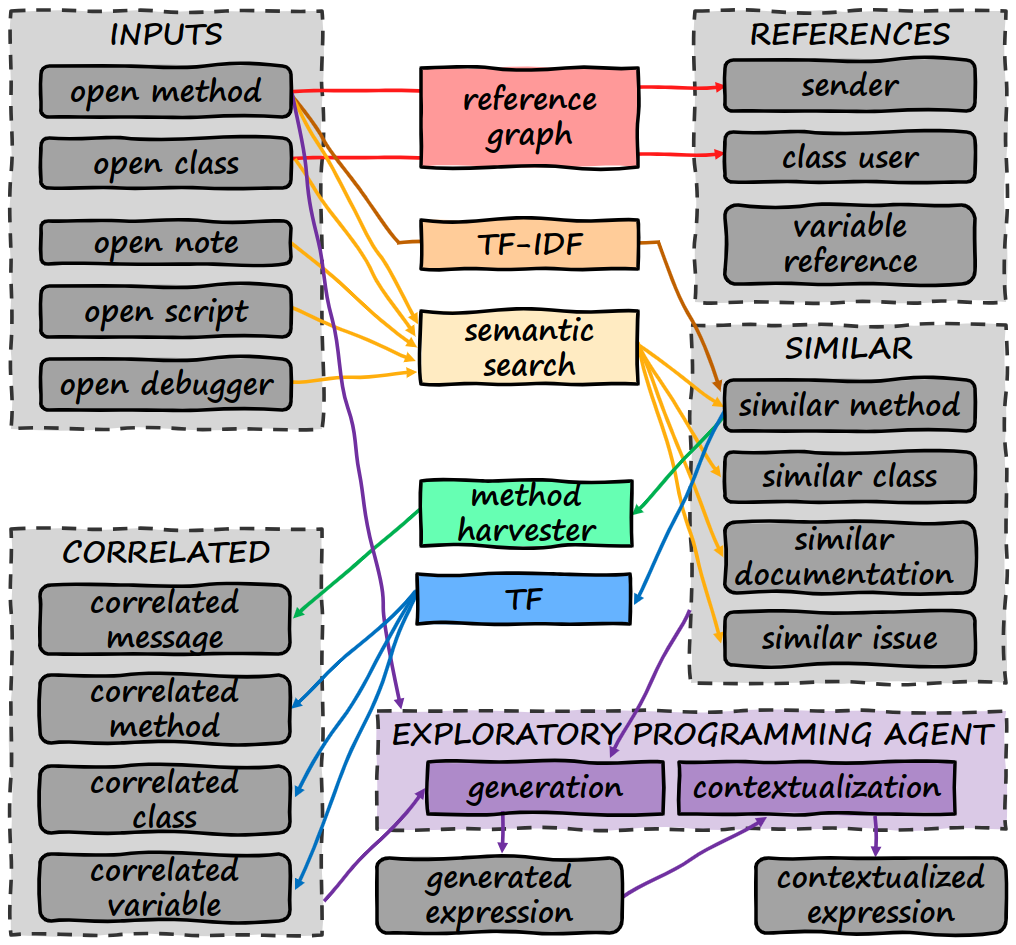
\includegraphics[width=\textwidth]{01_overview/graph.png}
	\caption[TODO]{
		TODO
	}
	\label{fig:suggestions/overview/graph}
\end{figure}

The suggestion engine defines different types and roles of artifacts and different strategies for recording and linking different kinds of information from the programming system.

We distinguish between three groups of artifacts:

\begin{description}[noextralabelsep]
	\item[Input artifacts] are captured from the original exploratory session and experiments of the programmer.

	This includes code artifacts such as \emph{methods} and \emph{classes} that the programmer is browsing or editing, \emph{do-it scripts} that they are writing or executing, and other types of information such as \emph{to-do lists} and \emph{bug reports} that they are interacting with.

	\item[Retrieved artifacts] refer to any piece of information that is available in the programming system and has been identified by the suggestion engine as potentially relevant for the next steps of the programmer's research process.

	Most retrieved artifacts relate to the implementation of systems: \emph{users} of code artifacts such as message senders, class users, and variable references provide context about their tasks and interfaces.
	\emph{Similar code artifacts} exemplify how other methods and classes solve related problems, use similar protocols, or implement similar interfaces.
	From the later, \emph{correlated code artifacts} can be extracted to summarize common building blocks of similar solutions, such as frequently sent messages, executed methods, instantiated classes, and references variables.
	A programmer who is editing a method has a higher statistical probability to use some of these correlated artifacts.

	Beyond code artifacts, the suggestion engine might also find \emph{documentation artifacts}, \emph{revision notes}, \emph{bug reports}, or other forms of communications from information sources that are related to the development of the software system.
	% todo: emphasize anywhere again that browsing is experiment?

	\item[Generated artifacts] are newly synthesized experiments from the suggestion engine.

	This includes generated and contextualized \emph{code expressions} based on similar and correlated artifacts.
	Generated code expressions can range from single message sends to entire class definitions and method implementations.
	However, the suggestion engine might also generate other types of artifacts to outline cluttered implementations, summarize long documentation artifacts, or suggest a list of steps to debug an error based on prior developer communications.
\end{description}

For each suggestable role of artifact, the suggestion engines defines one or multiple strategies that process and combine prior artifacts and produce new artifacts.
For example, we implement multiple strategies for searching similar methods based on their intentions and interface usage, provide different ways to extract correlated messages from methods based on static and dynamic call graphs, and employ different LLMs and heuristics through the exploratory programming agent for combining retrieved artifacts into new code expressions.
\Cref{fig:suggestions/overview/graph} provides an overview of all available types of artifacts and strategies in our prototype.
